%\documentclass[gray]{beamer}

%\documentclass[notes]{beamer}       % print frame + notes
%\documentclass[notes=only]{beamer}   % only notes
\documentclass{beamer}              % only frames


% to make notes
\usepackage{pdfcomment}
\newcommand{\pdfnote}[1]{\marginnote{\pdfcomment[icon=note]{#1}}}


\usepackage{graphicx}
\usepackage{tikz}
\usepackage{mathtools}
\usepackage{amssymb}
\usepackage{cite}
\usepackage{hyperref}
% -- To use color white throughout the document
\usepackage{xcolor}
% - To include Greenely logo
\usepackage{textpos}
% - Algorithms --
\usepackage{algpseudocode}% http://ctan.org/pkg/algorithmicx
\usepackage[titlenumbered,ruled]{algorithm2e}
\usepackage{algcompatible}
%
% - Python code --
\usepackage{listings}
%  ----
\usetikzlibrary{positioning}
\usepackage[swedish,english]{babel}
\title[Exploiting Temporal Difference for Energy Disaggregation via Discriminative Sparse Coding] % (optional, only for long titles)
{Exploiting Temporal Difference for Energy Disaggregation via Discriminative Sparse Coding}
\mode<presentation>{}
\author[Eric Leijonmarck]{
\includegraphics[height=2cm,width=2cm]{./figures/KTH.pdf}\\Eric Leijonmarck\\ Inspired by paper by Kotler et al.}

\institute[Royal Institute of Technology - Stockholm]
{
  \inst{}%{1}%
  Examiner: Timo Koski\\
  
\includegraphics[scale=0.3]{./figures/greenelylogolitteblack}
}
\date % (optional)

\AtBeginSection[]
{
	\begin{frame}<beamer>
		\frametitle{Table of Contents}
		\tableofcontents[currentsection,sectionstyle=show/hide]
	\end{frame}
}

\usepackage{xcolor}
\usepackage{wasysym}
\newcommand\crule[3][black]{\textcolor{#1}{\rule{#2}{#3}}}
\newcommand*{\vpointer}{\color{gray}\vcenter{\hbox{\scalebox{2}{\Huge\pointer}}}}

% used for qoutes
\usepackage{epigraph}

\begin{document}
\lstset{language=Python}          % Set your language (you can change the language for each code-block optionally)

%   ---   To make the group totally black ---
\bgroup
\newcommand{\norm}[1]{\left\lVert#1\right\rVert}

\setbeamercolor{itemize/enumerate body}{fg=white}
\setbeamertemplate{navigation symbols}{}
\color{white}

%\setbeamercolor{abstract,abstract title,alerted text,author,author in head/foot,author in sidebar,background,background canvas,bibliography entry author,bibliography entry location,bibliography entry note,bibliography entry title,bibliography item,block body,block body alerted,block body example,block title,block title alerted,block title example,button,button border,caption,caption name,date,date in head/foot,date in sidebar,description item,enumerate item,enumerate subitem,enumerate subsubitem,example text,fine separation line,footline,framesubtitle,frametitle,frametitle right,headline,institute,institute in head/foot,institute in sidebar,item,item projected,itemize item,itemize subitem,itemize subsubitem,itemize/enumerate body,itemize/enumerate subbody,itemize/enumerate subsubbody,local structure,logo,lower separation line foot,lower separation line head,math text,math text displayed,math text inlined,middle separation line foot,middle separation line head,mini frame,navigation symbols,navigation symbols dimmed,normal text,normal text in math text,normal text in math text,page number in head/foot,palette primary,palette quaternary,palette secondary,palette sidebar primary,palette sidebar quaternary,palette sidebar secondary,palette sidebar tertiary,palette tertiary,part name,part title,qed symbol,quotation,quote,section in head/foot,section in sidebar,section in sidebar shaded,section in toc,section in toc shaded,section name,section number projected,section title,separation line,sidebar,sidebar left,sidebar right,structure,subitem,,subitem projected,subsection in head/foot,subsection in sidebar,subsection in sidebar shaded,subsection in toc,subsection in toc shaded,subsection name,subsection number projected,subsection title,subsubitem,subsubitem projected,subsubsection in head/foot,subsubsection in sidebar,subsubsection in sidebar shaded,subsubsection in toc,subsubsection in toc shaded,subsubsection number projected,subtitle,title,title in head/foot,title in sidebar,titlegraphic,titlelike,upper separation line foot,upper separation line head,verse}{fg=white}

% --- Set color of presentation to white ----
\setbeamercolor{background canvas}{bg=black}
\setbeamercolor*{frametitle}{fg=white,bg=black}
\setbeamercolor{date in head/foot}{fg=white}
\setbeamercolor{section in head/foot}{fg=white}
\setbeamercolor{section in toc}{fg=black,bg=white}
\setbeamercolor{alerted text}{fg=white}
\setbeamercolor{section in toc}{fg=white}
\setbeamercolor*{structure}{fg=white}
\setbeamercolor*{title}{fg=white}
\setbeamercolor*{author}{fg=white}
\setbeamercolor*{institute}{fg=white}
\setbeamercolor*{date}{fg=white}
\setbeamercolor*{itemize}{bg=white,fg=white}




% - add the logo of Greenely to each of the pages
\addtobeamertemplate{frametitle}{}{%
\begin{textblock*}{200mm}(.85\textwidth,-1cm)

\includegraphics[height=2cm,width=2cm]{./figures/KTH.pdf}
\end{textblock*}}

% to remove the figure caption of a figure
\setbeamertemplate{caption}{\insertcaption} 

% Presentation
% Show a well disposed report, with clear accounts of the project and the results, clear analysis, and well founded argumentation, as well as good language usage, format and scientific accuracy. Show a good ability to orally present with clear argumentation and analysis, and also a good ability to discuss the work.
%%%%%%%%%%%%%%%%%%%%%%%%%%%%%%%
\frame{\titlepage}
%{Greenely}
%{Energy disaggregation, informatics task related to energy efficiency}
%{Discriminative, conditional models}
%{Sparse Coding, Neural Networks}
%{Appliance-level data could reduce consumption by 12\%}
%\{"Smart Meters", collect whole-home level per hour}
%%%%%%%%%%%%%%%%%%%%%%%%%%%%%%

\begin{frame}<beamer>
		\frametitle{Table of Contents}
		\tableofcontents[currentsection]
\end{frame}

\section{Disaggregation; state of 2015}


\begin{frame}
\frametitle{State of 2015}
\framesubtitle{Why}
\begin{itemize}
	\item {Rising Energy Consumption}
	\item{Energy Problems often Informatics Problem}
	\item{Energy Disaggregation}
	\item{Receiving Information, less energy}
\end{itemize}


\end{frame}
%%%%%%%%%%%%%%%%

%%%%%%%%%%%%%%%%
\begin{frame}
	\frametitle{State of 2015}
	\framesubtitle{Challenge}
		\begin{figure}[!ht]
			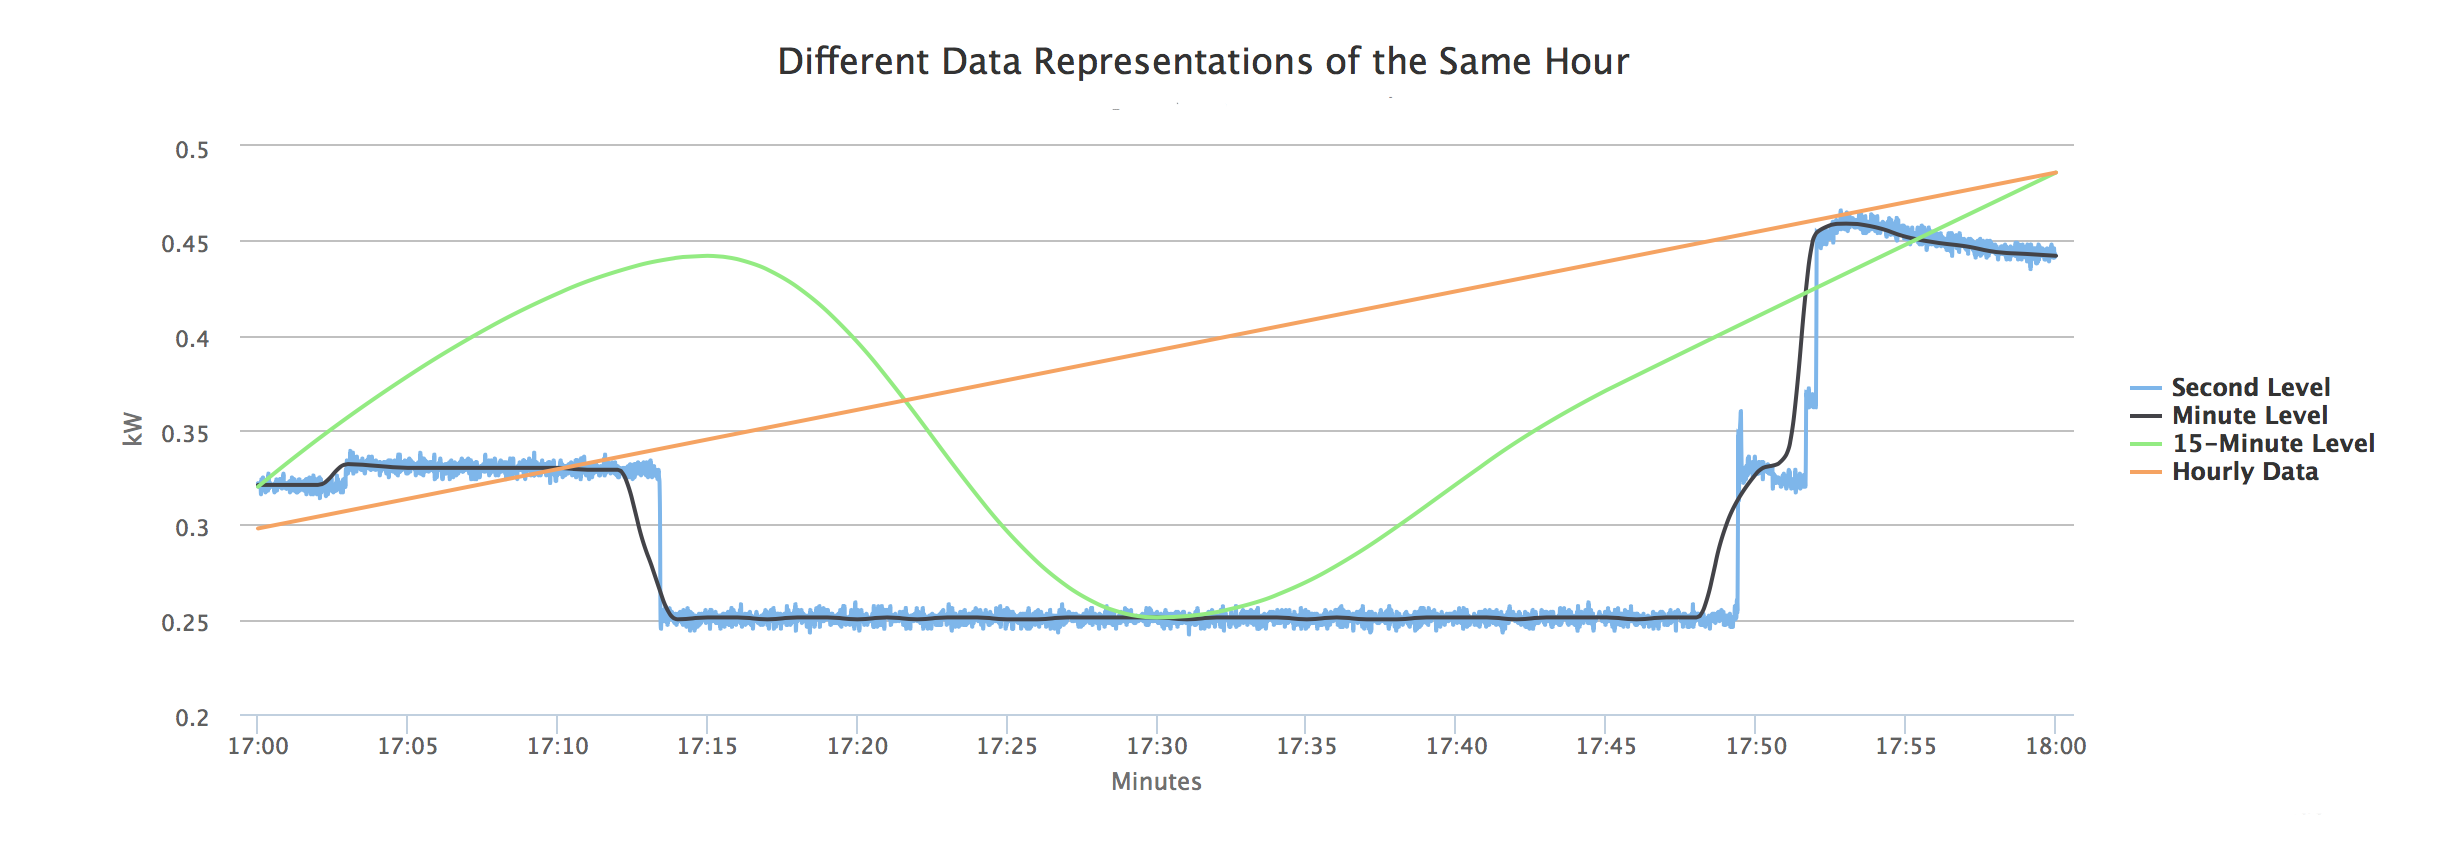
\includegraphics[scale=0.22]{./figures/hourlyexamplefixed.png}
		\end{figure}
\end{frame}

%%%%%%%%%%%%%%%%


\begin{frame}
	\frametitle{State of 2015}
	\framesubtitle{Challenge}
	\begin{itemize}
		\item{Challenge}
		\begin{figure}[!ht]
			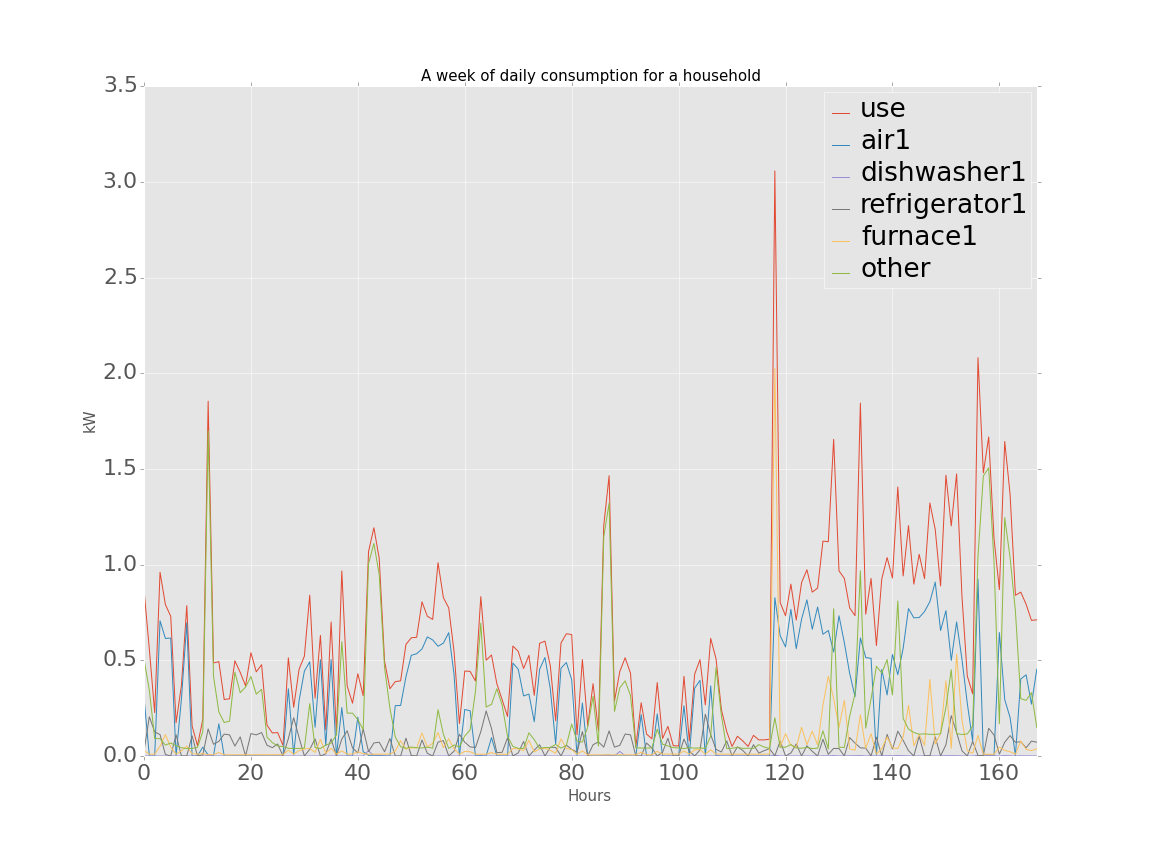
\includegraphics[scale=0.18]{./figures/weekconsump}
		\end{figure}
	\end{itemize}

\end{frame}
%%%%%%%%%%%%%%%%

\begin{frame}
	\frametitle{State of 2015}
	\framesubtitle{Research}
	\begin{itemize}
		\item{Research in Energy Disaggregation}
	\end{itemize}
	\begin{figure}[!ht]
		\colorbox{white}{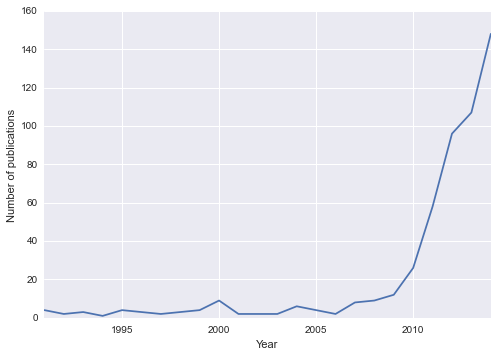
\includegraphics[scale=0.40]{./figures/growth}}
	\end{figure}
		Increase at 2010 from 20 - 140 in 4 years
\end{frame}

%%%%%%%%%%%%%%%%%
\begin{frame}
	\frametitle{State of 2015}
	\framesubtitle{Solution}
	\begin{itemize}
		\item{Ed Freeman, More Data or Better Algorithms?}
		\begin{enumerate}
			\item{Having a good problem to work on}
			\item{Having a good approach to that problem}
			\item{Having decent data. Quality is much more important than quantity}
			\item{Handling the data well -- good transforms, good missing value handling, making sure that all approaches make sense for the problem.}
		\end{enumerate}
	\end{itemize}
	\epigraph{Not everything that can be counted counts, and not everything that counts can be counted.}{Albert Einstein}
\end{frame}
%%%%%%%%%%%%%%%%
\begin{frame}
	\frametitle{Project Goal}
		\begin{itemize}
			\item{Implement the Discriminative Disaggregation algorithm using Sparse Coding}
			\item{Having it work on the dataset provided by PecanStreet}
			\item{Try to exploit temporal differences, since Kotler did not take that into account}
		\end{itemize}
\end{frame}
%%%%%%%%%%%%%%%%
%%%%%%%%%%%%%%%%%%%%%%%%%%%%%%
\section{Pre-Processing Data}
%%%%%%%%%%%%%%%%%%%%%%%%%%%%%%%%%
\begin{frame}
\frametitle{Input}
\framesubtitle{We have $1:k$ appliances}
\begin{itemize}
\item{We define one class (e.g. heater) $\mathbf{X}_i \leftarrow 1,\dots, k$}
\item{Where $\mathbf{X}_i \in \mathbb{R}^{T \times m}$, $T$ hourly week data for $m$ houses}
\item{\textbf{One} aggregated household $\bar{\mathbf{X}} \leftarrow \sum_{i:k} \mathbf{X}_i$}
\item{Assuming we have individual energy readings $\mathbf{X}_1,\dots,\mathbf{X}_k$}
\item{Goal: test with new data $\bar{\mathbf{X}}'$ to components $\mathbf{X}_1',\dots,\mathbf{X}_k'$}
\end{itemize}
\end{frame}
%%%%%%%%%%%%%%%%%%%%%%%%%%%%%%
\begin{frame}
\frametitle{Input data}
\framesubtitle{We have $1:k$ appliances}
\centering
\begin{equation*}
\underbrace{\mathbf{X}_i \in \mathbb{R}^{T \times m}}
\end{equation*}

\begin{equation*}
\begin{bmatrix}
\text{App} & \mathbf{x}_1^{(j)} & \cdots & & \mathbf{x}_1^{(m)}\\
1h & 0.8 kWh & \cdot & & \cdot \\
2h & 0.7 kWh & \cdot & & \cdot \\
\vdots & \vdots & \cdot & & \cdot \\
168h & 0.1kWh & \cdot & &  \cdot
\end{bmatrix}
\end{equation*}
\textit{How do we get this format?}
\end{frame}
%%%%%%%%%%%%%%%%%%%%%%%%%%%%%
\begin{frame}
	\frametitle{Pre-processing raw-data}
	\begin{itemize}
		\item{Number of missing values in data}
		\item{When missing - what to do?}
		\item{Demonstation of processing}
	\end{itemize}
\end{frame}
% - Nested pretraining using the components of the trained training samples
%%%%%%%%%%%%%%%%%%%%%%%%%%%%%%%%%%%%%%%%%%%%%%%%
\section{Preliminaries}
%%%%%%%%%%%%%%%%%%%%%%%%%%%%%%%%%%%%%%%%%%%%%%%%%
\begin{frame}
	\frametitle{Fundamentals}
	\begin{itemize}
		\item{Optimization, cost/penalty function}
		\item{Machine Learning}
		\begin{itemize}
			\item {SupervisedLearning \& Unsupervised Learning}
			\item{Dimensionality Reduction, PCA \& Autoencoders}
			\item{Artificial Neural Networks, Deep Learning, Sparse-Coding}
		\end{itemize}
	\end{itemize}
	\note{The goal is to find the models that represent the input well; and the loss function quantifies the amount of deviation of the prediction from the true values!
		standard form is often referred to as a cost or loss function that maps events or values of variables to some value that represents the ”cost” involving that particular event. In classification, the cost is usually portrayed as ”penalty” involving an incorrect classification.
		ML: the study of algorithms that can learn from data}
\end{frame}

%%%%%%%%%%%%%%%%%%%%%%%
\begin{frame}
\frametitle{Machine Learning}
\begin{columns}[T] % align columns
	\begin{column}{.28\textwidth}
%		\color{red}\rule{\linewidth}{4pt}
		\crule[white]{3cm}{3cm}  
		
		\qquad \color{white}{Raw Data}
	\end{column}%
	$\vpointer$
	\hfill%
	\begin{column}{.28\textwidth}
		\crule[yellow]{3cm}{3cm}
		
		\qquad  \color{yellow}{Features}
	\end{column}%
	$\vpointer$
	\hfill
	\begin{column}{.28\textwidth}
		\crule[red!50!white!100]{3cm}{3cm}
		
		\qquad  \color{red!50!white!100}Models
	\end{column}%
\end{columns}
\note{
	Data -> point cloud in feature space
	Feature = Numerica representation of raw data,
	Model = mathematical "summary" of features
	How do you make something that works = choose the right model and features, given data and task
	
	Model, a geometric shape that best "fits" the point cloud}
\end{frame}

%%%%%%%%%%%%%%%%%%%%%%%
\begin{frame}
	\frametitle{Super/Unsupervised learning}
	\begin{figure}
		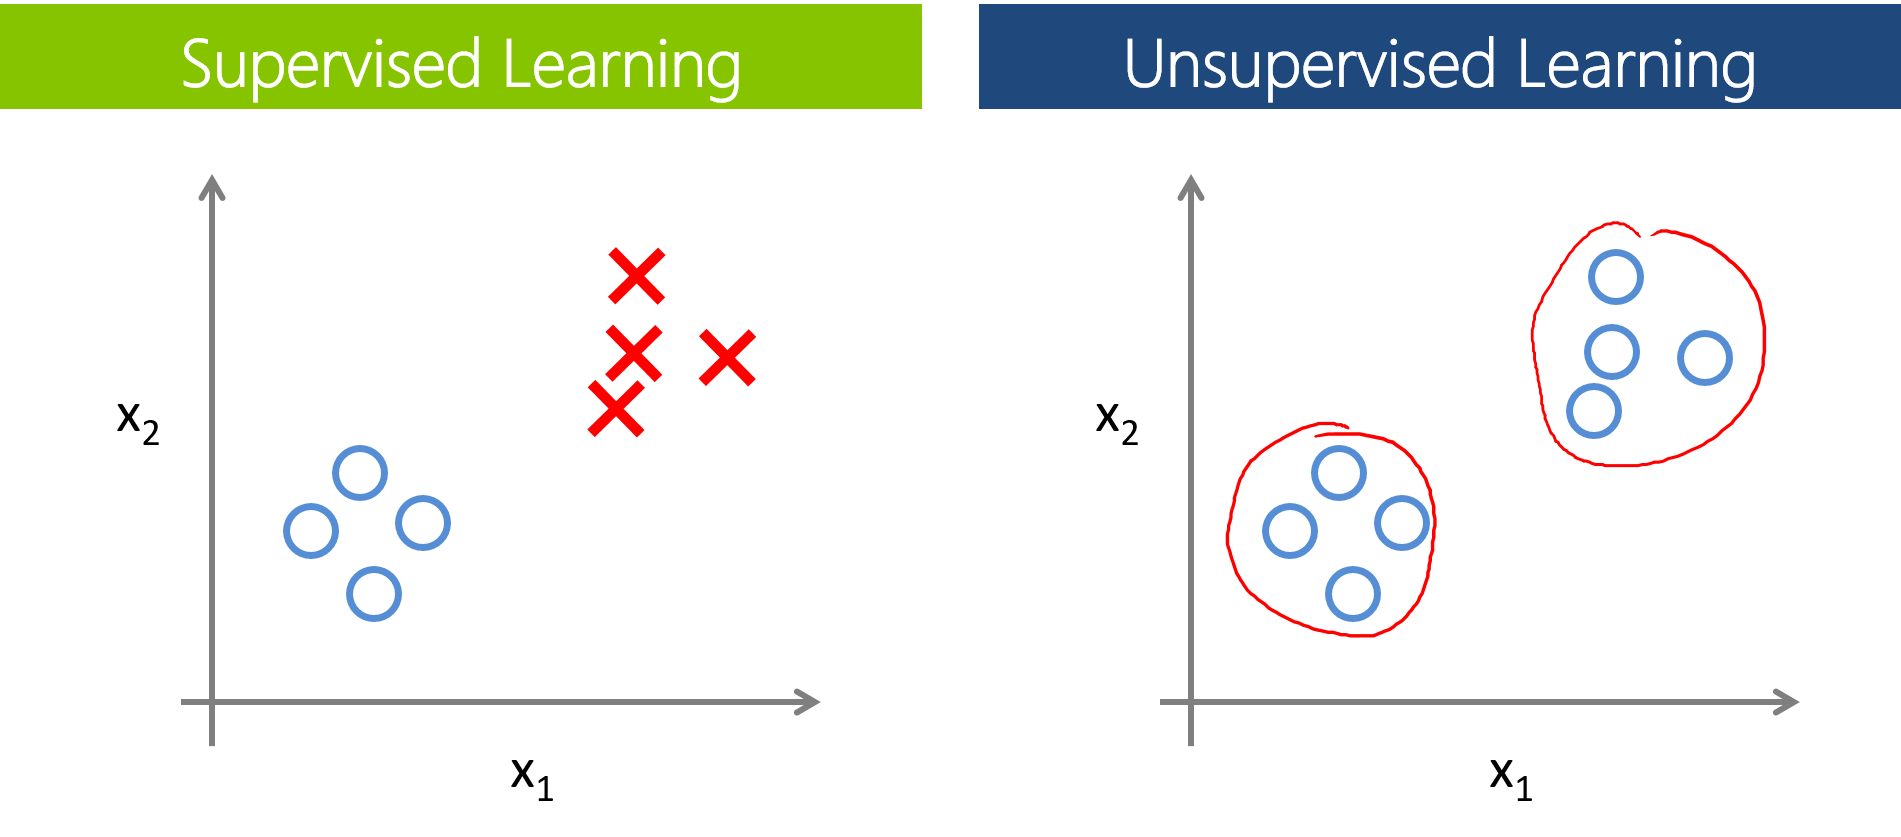
\includegraphics[scale=0.33]{./figures/super_unsupervised.png}
	\end{figure}
	\note{Machine Learning is a class of algorithms which is data-driven, i.e. unlike "normal" algorithms it is the data that "tells" what the "good answer" is. Example: a hypothetical non-machine learning algorithm for face recognition in images would try to define what a face is (round skin-like-colored disk, with dark area where you expect the eyes etc). A machine learning algorithm would not have such coded definition, but would "learn-by-examples": you'll show several images of faces and not-faces and a good algorithm will eventually learn and be able to predict whether or not an unseen image is a face.
		
		This particular example of face recognition is supervised, which means that your examples must be labeled, or explicitly say which ones are faces and which ones aren't.
		
		In an unsupervised algorithm your examples are not labeled, i.e. you don't say anything. Of course, in such a case the algorithm itself cannot "invent" what a face is, but it can try to cluster the data into different groups, e.g. it can distinguish that faces are very different from landscapes, which are very different from horses.
		
		Since another answer mentions it (though, in an incorrect way): there are "intermediate" forms of supervision, i.e. semi-supervised and active learning. Technically, these are supervised methods in which there is some "smart" way to avoid a large number of labeled examples. In active learning, the algorithm itself decides which thing you should label (e.g. it can be pretty sure about a landscape and a horse, but it might ask you to confirm if a gorilla is indeed the picture of a face). In semi-supervised learning, there are two different algorithms which start with the labeled examples, and then "tell" each other the way they think about some large number of unlabeled data. From this "discussion" they learn.
		
		}
\end{frame}

%%%%%%%%%%%%%%%%%%%%%%%%%%%%%%%%%%%%%%%%%%%%%%%%
\begin{frame}
	\frametitle{Autoencoders \& PCAs}
	\begin{figure}[H]
		\begin{minipage}{.45\textwidth}
			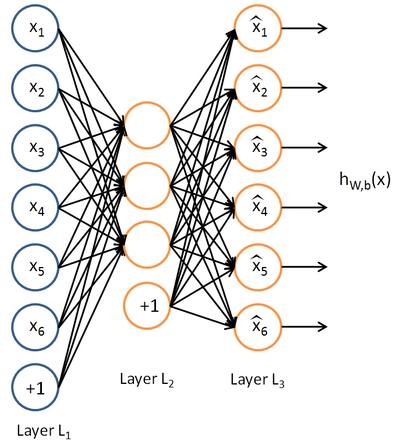
\includegraphics[width=.98\linewidth]{./figures/autoencoder.png}
		\end{minipage}
		\begin{minipage}{.45\textwidth}
			\begin{equation*}
			\norm{\mathbf{A}\sigma(\mathbf{A}^T \mathbf{x}) - \mathbf{x}}^2
			\end{equation*}
		\end{minipage}
		\caption{The figure gives a comparison for the trained model for both Kotler. et.al. and the model predicted by the method in this thesis.}
	\end{figure}
	\note{The goal is to find the models that represent the input well; and the loss function quantifies the amount of deviation of the prediction from the true values!
		standard form is often referred to as a cost or loss function that maps events or values of variables to some value that represents the ”cost” involving that particular event. In classification, the cost is usually portrayed as ”penalty” involving an incorrect classification.
		ML: the study of algorithms that can learn from data
		
		
		we want to represent the signal as best as we can with the expression below by giving the values for matrix A as best as possible
		}
\end{frame}
%%%%%%%%%%%%%%%%%%%%%%%%%%%%%%%%%%%%%%%%%%%%%%%%
\begin{frame}
	\frametitle{Deep Learning \& Sparse Coding}
	Sparse Coding (Olshausen \& Field, 1996) \\
	\textit{Input:} \\
	Data $\mathbf{x}^{(1)}, \mathbf{x}^{(2)}, \dots, \mathbf{x}^{(m)}$, (each in $\mathrm{R}^{m\times n}$) \\
	\vspace{0.2in}
	\textit{Learn:} \\
	Dictionary of bases $\theta_1,\theta_2,\dots,\theta_k$, each input can be approximately decomposed as: \\
	$\begin{matrix}
		\text{ } &&& \mathbf{x} \approx \sum_{j=1}^k a_j \theta_j \\
		\text{where} &&& a_j \text{ are mostly zeros (sparse)}
	\end{matrix}$
	\note{Introduced sparse-coding and connected it to
		neural-science. How did neurals in the visual
		get the type of receptive field properties,
		and they tried to connect it to optimization problem that they believed that neurans were trying to solve.
		}
\end{frame}
%%%%%%%%%%%%%%%%%%%%%%%%%%%%%%%%%

\begin{frame}
	\frametitle{Deep Learning \& Sparse Coding}
	Natural Images \hspace{0.5in} Learned bases ($\theta_1,\dots,\theta_{64}$):
	\begin{figure}
		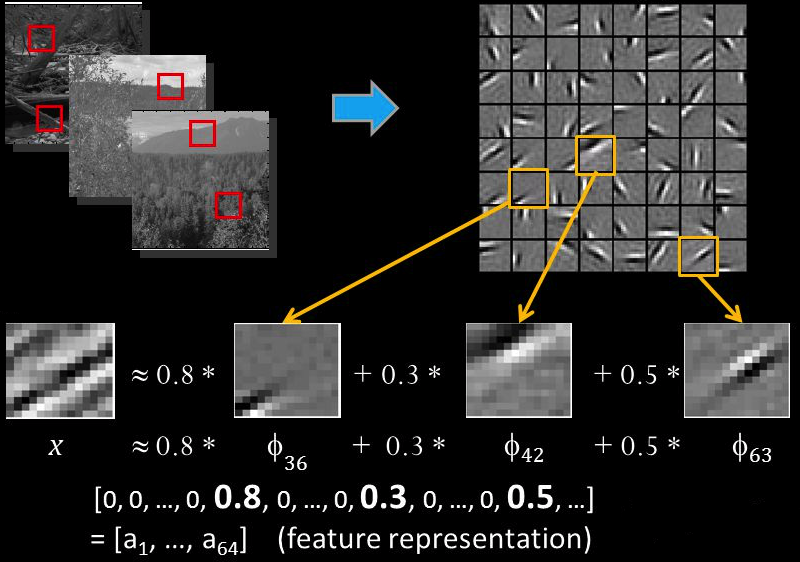
\includegraphics[scale=0.4]{./figures/sparse_second.png}
	\end{figure}
	\note{
		Break the iamges into patches,
		Imagine the natural images as a collection of vectors of small pieces of the images.
		These were then asked to basis that had a sparse representation which indeed gives a very resemblence of the image.
		
		You could do the singular value decomposition (directions that explain as much of the variance of the vectors as possible),
		but got noicy and extremely dense.
		
		Sparse-Coding is a neural plausible, efficient, take advantage of matrix multiplications.
		}
\end{frame}
%%%%%%%%%%%%%%%%%%%%%%%%%%%%%%%%%
\begin{frame}
	\frametitle{Deep Learning \& Sparse Coding}
	
	NonConvex Formulations
	\begin{equation*}
	\min_{a_i^{(j)},\phi_i}\sum_{j=1}^m
	\ \underbrace{\norm{\mathbf{x}^{(j)}-\sum_{i=1}^ka_i^{(j)}\phi_i}^2}_{\text{reconstruction term}}+\underbrace{\lambda \sum_{i=1}^k
		S(a_i)^{(j)}}_{\text{sparsity penalty}}
	\end{equation*}
	This optimization technique is \textcolor{red}{\textbf{NP-hard}}, can have many local optima; but \textcolor{red}{\textbf{heuristics}} work well empirically.

	\note{
		You check how much you havent explained with the learned basis and activations,
		but you want them to be sparse.
		Therefore you add the non-linear penalty function, encourages sparsity
	}
\end{frame}
%%%%%%%%%%%%%%%%%%%%%%%%%%%%

\begin{frame}
	\frametitle{Deep Learning \& Sparse Coding}
	This network performs a \textcolor{red}{gradient descent} by alternating between:
	\begin{enumerate}
		\item { $  r \quad \LHD \quad b - Ax$}
		\item{$ x \quad  \LHD \quad  x + \nu (A^T r - \nabla L(x))$}
	\end{enumerate}
	
	\begin{figure}
		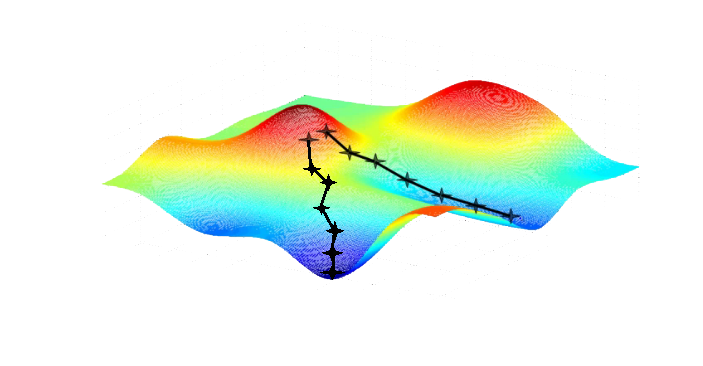
\includegraphics[scale=.5]{./figures/gradient_descent_transparent.png}
	\end{figure}
	\note{
		current representation and current basis, calc residual
		update sparse representation is, 
		method for outputting a sparse code
	}
\end{frame}
%%%%%%%%%%%%%%%%%%%%%%%%%%%%

\begin{frame}
	\frametitle{Deep Learning \& Sparse Coding}
	
	Remember from the Autoencoder slide,
	\begin{equation*}
	\label{eq:auto}
	\norm{\mathbf{A}\sigma(\mathbf{A}^T \mathbf{x}) - \mathbf{x}}^2, \quad
	\mathbf{B} = \sigma(\mathbf{A}^T \mathbf{x})
	\end{equation*}
	Instead we think of it as a neural implementation, the basic idea of the Discriminative Disaggregation Sparse Coding algorithm.
	\begin{equation*}
	\arg \! \min_{A \geq 0} \norm{\mathbf{X}_i - \mathbf{B}_i\mathbf{A}}_F^2 + \underbrace{\lambda \sum_{p,q} \mathbf{A}_{pq}}_{\text{added sparsity}}
	\end{equation*}
	$\mathbf{A},\mathbf{B}$ are neural encoders as layers of neuronal synapses. Where the learning comes into $\mathbf{A}$.
	\note{
		bajs 
	}
\end{frame}
%%%%%%%%%%%%%%%%%%%%%%%%%%%%


\begin{frame}
\frametitle{Sparse coding pre-training}
\framesubtitle{pre-train activations and basis vectors}
\begin{algorithm}[H]
\caption{Dicriminative disaggregation sparse coding}
\SetKwInOut{Input}{input}
\Input{data points for each individual source $\mathbf{X}_i \in
\mathbb{R}^{T \times m}, i = 1:k,$ regularization $\lambda
\in \mathbb{R}_+$, with gradient step size $\alpha \in \mathbb{R}_+$.}
\begin{algorithmic}[1]
\Statex{  \textbf{Sparse coding pre-training:}}
\Statex{  \hspace{0.2in} 1. Initalize \textbf{B}$_i$, $\mathbf{A}_i ; \geq 0$, scale columns $\mathbf{B}_i$ s.t. $\norm{ \mathbf{b}_i^{(j)}}_2 =1$}
\Statex{ \hspace{0.2in} 2. For each $i=1,\dots,k,$ iterate until convergence: }
\Statex \hspace{0.4in} $\mathbf{A_i} \leftarrow \arg \! \min_{A \geq 0} \norm{\mathbf{X}_i - \mathbf{B}_i\mathbf{A}}_F^2 + \lambda \sum_{p,q} \mathbf{A}_{pq}$
\Statex \hspace{0.4in} $\mathbf{B}_i \leftarrow  \arg \! \min_{B \geq 0,\norm{\mathbf{b}^{(j)}}_2 \leq 1} \norm{\mathbf{X}_i - \mathbf{B} \mathbf{A}_i }_F^2$
\end{algorithmic}
\end{algorithm}
\end{frame}
% - Nested pretraining using the components of the trained training samples
%%%%%%%%%%%%%%%%%%%%%%%%%%%%%%%%%%%%%%%%%%%%%%%%
\begin{frame}
\frametitle{Discriminative disaggregation training}
\framesubtitle{perceptron algorithm}
\begin{algorithm}[H]
\caption{Dicriminative disaggregation sparse coding}
\label{alg:DDSC}
\begin{algorithmic}[1]
\Statex \textbf{Discriminative disaggregation training:}
\Statex  \hspace{0.2in} 3. Set $\mathbf{A}_{1:k}^* \leftarrow \mathbf{A}_{1:k},\hat{\mathbf{B}}_{1:k} \leftarrow \mathbf{B}_{1:k}.$
\Statex  \hspace{0.2in} 4. Iterate until convergence:
\Statex \hspace{0.4in} $\hat{\mathbf{A_{1:k}}} \leftarrow \arg \! \min_{A_{1:k} \geq 0} F\left( \bar{\mathbf{X}},\tilde{\mathbf{B}}_{1:k},\mathbf{A}_{1:k} \right)$
\Statex \hspace{0.4in} $\tilde{\mathbf{B}} \leftarrow \left[ \tilde{\mathbf{B}} - \alpha \left( (\bar{\mathbf{X}} - \tilde{\mathbf{B}}\hat{\mathbf{A}})\hat{\mathbf{A}}^T - (\bar{\mathbf{X}}-\tilde{\mathbf{B}}\mathbf{A}^*)(\mathbf{A}^*)^T \right) \right]_+$
\Statex \hspace{0.4in} $\forall \quad i,j,\mathbf{b}_i^{(j)} \leftarrow \mathbf{b}_i^{(j)} / \norm{\mathbf{b}_i^{(j)}}_2$
\Statex \textbf{Given aggregated test examples $\bar{\mathbf{X}}'$}
\Statex \hspace{0.2in} 5. $\hat{\mathbf{A}}'_{1:k} \leftarrow \arg \! \min_{\mathbf{A}_{1:k} \geq 0} F(\bar{\mathbf{X}}',\tilde{\mathbf{B}}_{1:k},\mathbf{A}_{1:k})$
\Statex \hspace{0.2in} 6. Predict $\hat{\mathbf{X}}_i' = \mathbf{B}_i\hat{\mathbf{A}}_i'$
\end{algorithmic}
\end{algorithm}
\note{Learning Structured Prediction Models: A Large Margin Approach}
\end{frame}

% - set basis and actibation as trained from pre-training
% - gradiant step-size
% - perceptron algorithm, updating tilde-B
% - Learning Structured Prediction Models: A Large Margin Approach

% - F : stands for the Frobeus norm

%%%%%%%%%%%%%%%%%%%%%%%%%%%%%%%%%%%%%%%%%%%%%%%%
% - total energy priors, we evaluate the norm (total energy) also
% - we lasso in the atoms and take out what is valuable by L2

%%%%%%%%%%%%%%%%%%%%%%%%%%%%%%%%%%%%%%%%%%%%%%%%%%
\section{Results and Extensions}
%%%%%%%%%%%%%%%%%%%%%%%%%%%%%%%%%%%%%%%%%%%%%%%

\begin{frame}
\frametitle{Facts}
\begin{itemize}
	\item{Kotler Dataset 590 homes, two years. 52 device types.}
	\item {\textbf{Raw} Data from 2014 and 2015, 8 billion readings, from 21 appliances, 689 houses.}
	\item{\textbf{Cleaned} Data 213 houses}
	\item{Each run (9 runs total excluding grid search) ranged from 4 hours to 24 hours on a 46 GB Ram, quadro Core CPU ( Core i7-4790-processor)}
\end{itemize}
\end{frame}

%%%%%%%%%%%%%%%%%%%%%%%%%%%%%%%%%%%%%%%

\begin{frame}
	\frametitle{Trained models}
	\framesubtitle{Basis Functions}
	\begin{figure}[H]
		\centering
		\begin{minipage}{.5\textwidth}
			\centering
			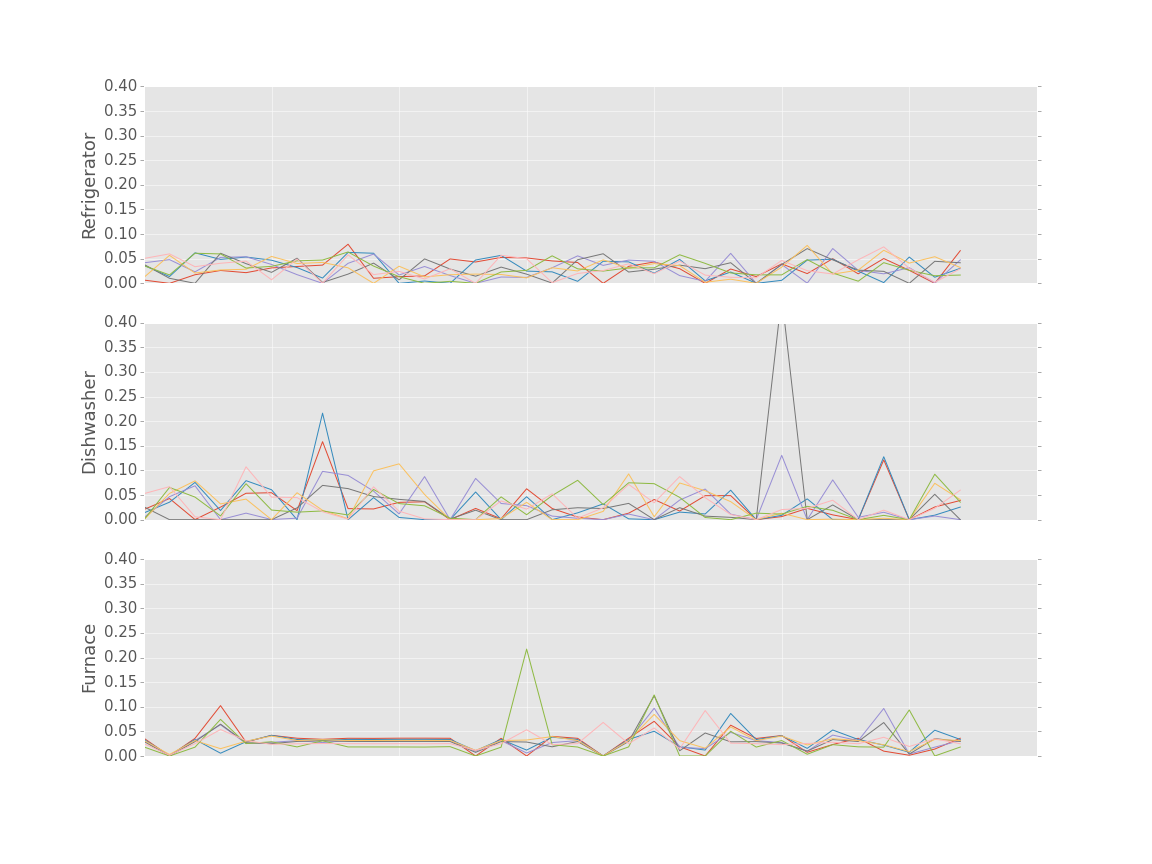
\includegraphics[scale=0.16]{./figures/app_basis_transparent.png}
		\end{minipage}%
		\begin{minipage}{.5\textwidth}
			\centering
			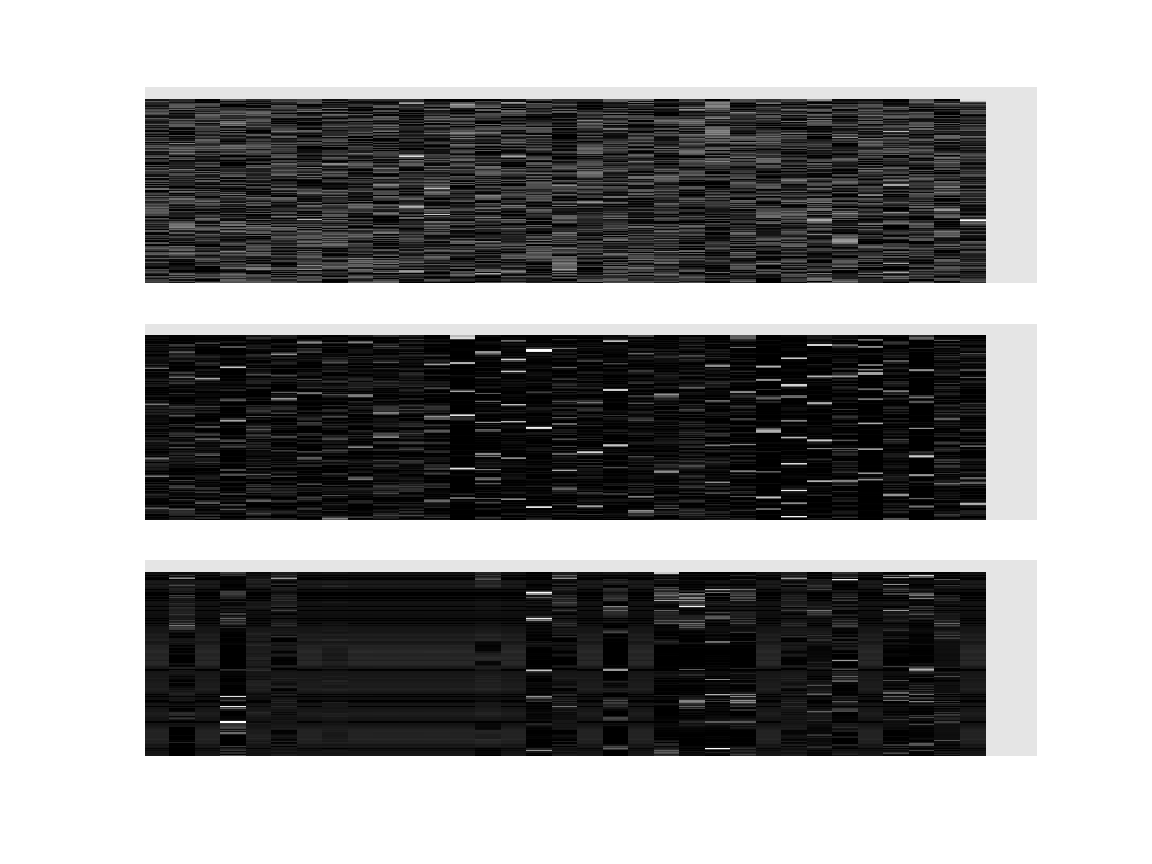
\includegraphics[scale=0.16]{./figures/basis_transparent.png}
		\end{minipage}
		\caption{The figure gives a comparison for the trained model for both Kotler. et.al. and the model predicted by the method in this thesis.}
	\end{figure}
	\note{
		The right plots show that the refrigerator is ”on” most of the time but with low power as we can see that the plot has mostly grey and some black in it. We can see that the dishwasher has peaked behavior in that some of the basis are almost pure white and some are black. We find interesting behaviors in the representations of the furnace as some of the basis fucntions really do look the same indicating that some furnaces behave similar and in similar magnitude.
}
\end{frame}
%%%%%%%%%%%%%%%%%%%%%%%%%%%%%%%%%%%%%%%%%%%%%%%
\begin{frame}
\frametitle{Trained models}
\framesubtitle{DDSC}
\begin{figure}[H]
\centering
\begin{minipage}{.5\textwidth}
	\centering
	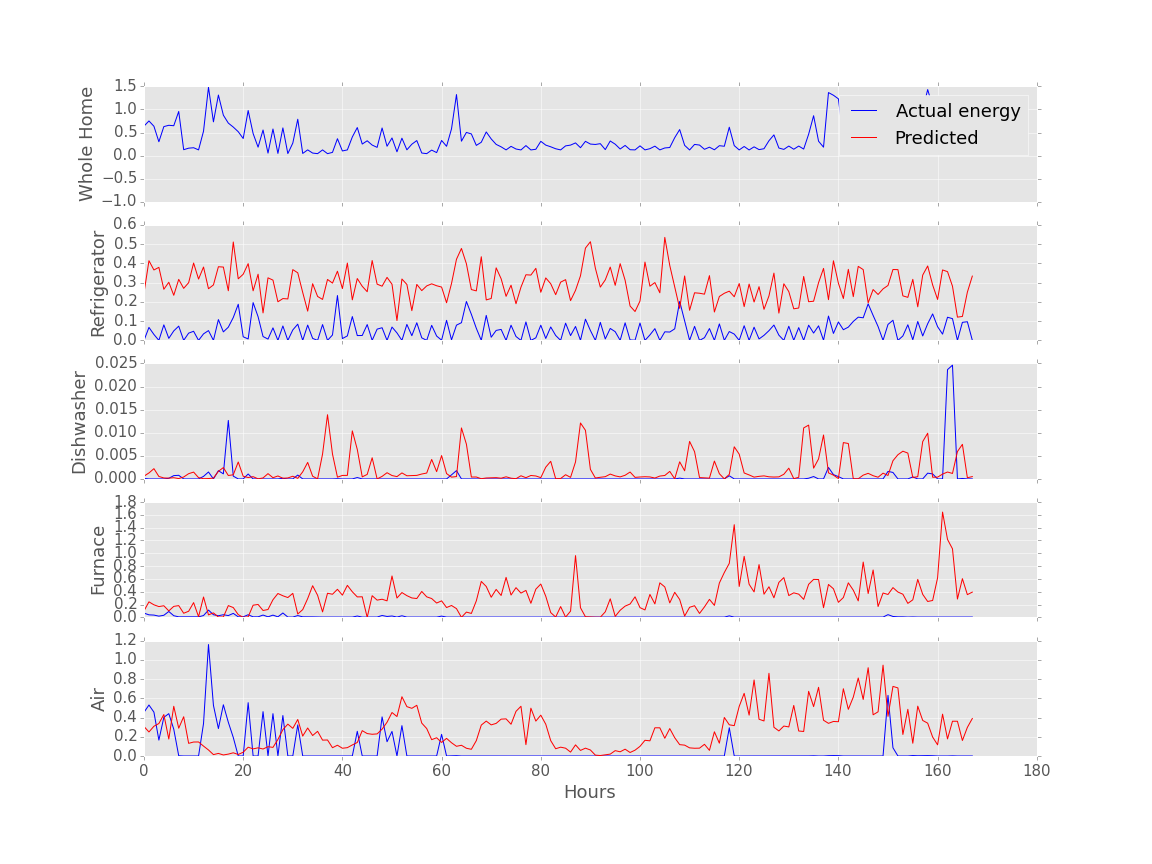
\includegraphics[width=.9\linewidth]{./figures/appliances.png}
\end{minipage}%
\end{figure}
\note{
	
	}
\end{frame}
%%%%%%%%%%%%%%%%%%%%%%%%%%%%%%%%%%%%%%%%%%%%%%%
\begin{frame}
	\frametitle{Exploiting temporal difference}
	\framesubtitle{Results}
	\begin{figure}[H]
		\centering
		\begin{minipage}{.3\textwidth}
			\centering
			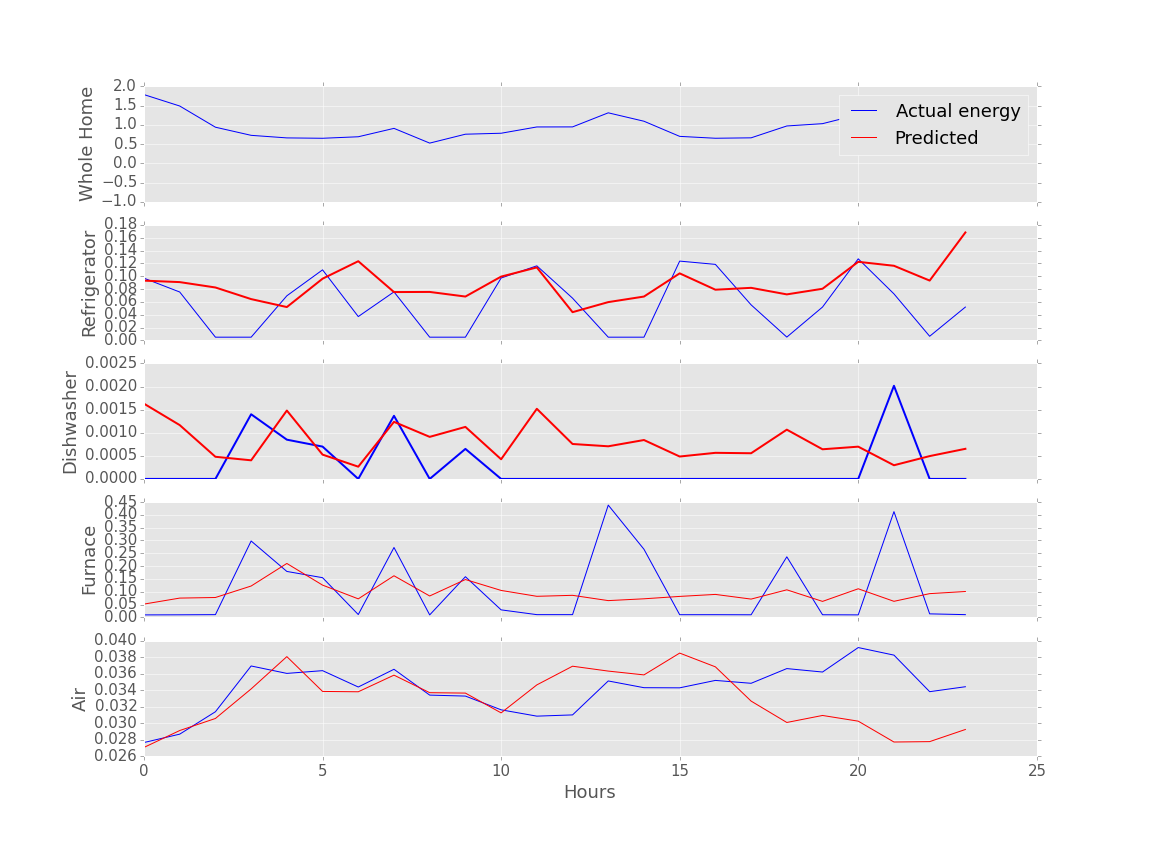
\includegraphics[scale=0.09]{./figures/normal_250_24.png}
		\end{minipage}%
		\begin{minipage}{.3\textwidth}
			\centering
			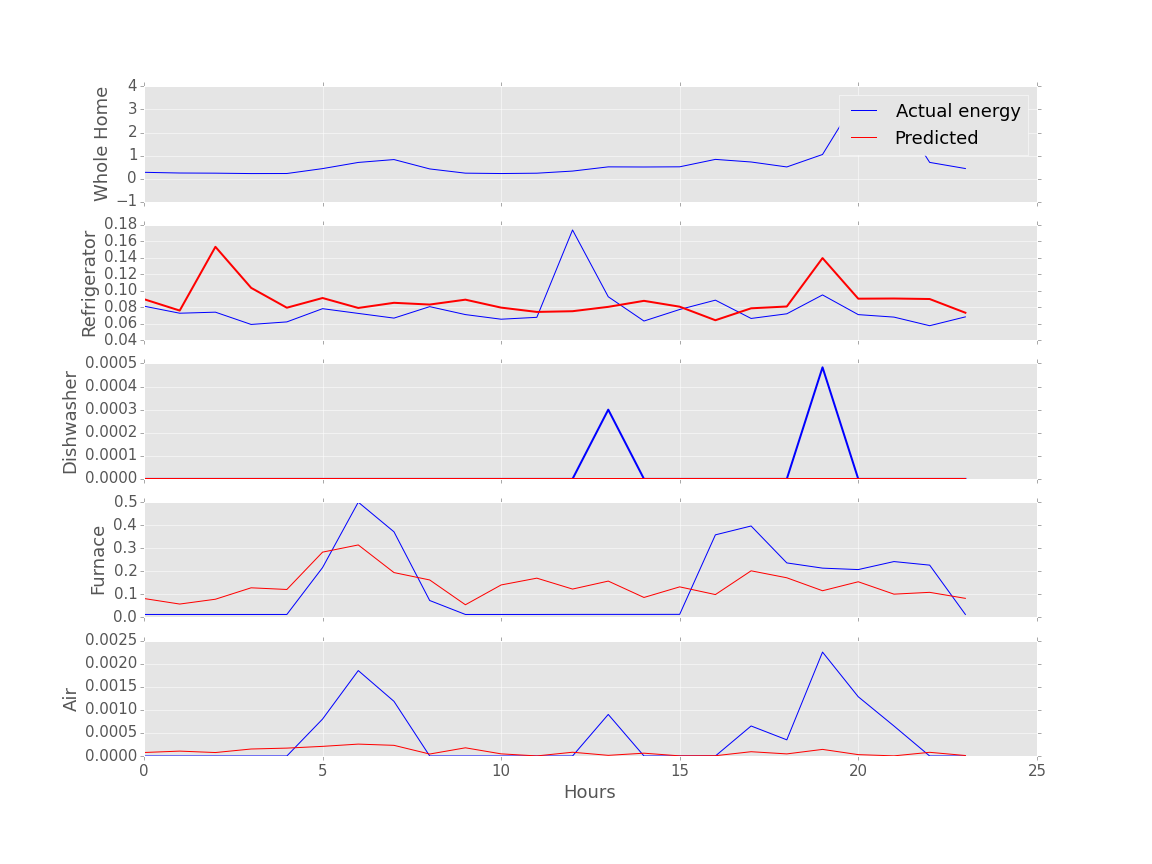
\includegraphics[scale=0.09]{./figures/days_250_24.png}
		\end{minipage}
		\begin{minipage}{.3\textwidth}
			\centering
			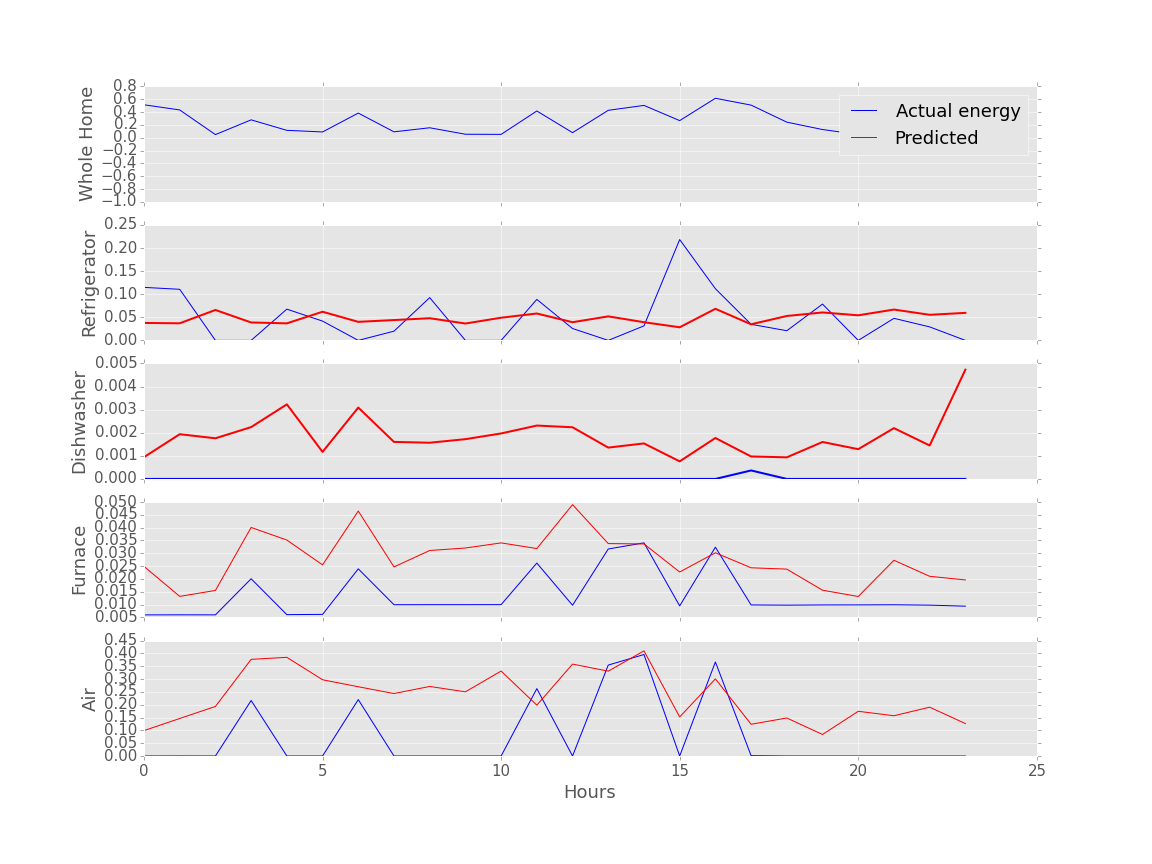
\includegraphics[scale=0.09]{./figures/end_250_24.png}
		\end{minipage}
	\end{figure}
	\note{
		Interesting to note is that the algorithm has found some of the energy profiles of some appliances. Looking at the plot to the bottom left we see that the prediction has actually been proved to be almost in line with the true profile for 10 of the data points (10 hours). We can also see that the algorithm can output completely different profiles by looking at the refrigerator for the weekdays dataset compared to that of the air-condition profile for the week dataset.
		}
\end{frame}
%%%%%%%%%%%%%%%%%%%%%%%%%%%%%%%%%%%%%%%%%%%%%
\begin{frame}
	\frametitle{Activations and Basis Norm of DDSC algorithm}
	\framesubtitle{Results}
	\centering
	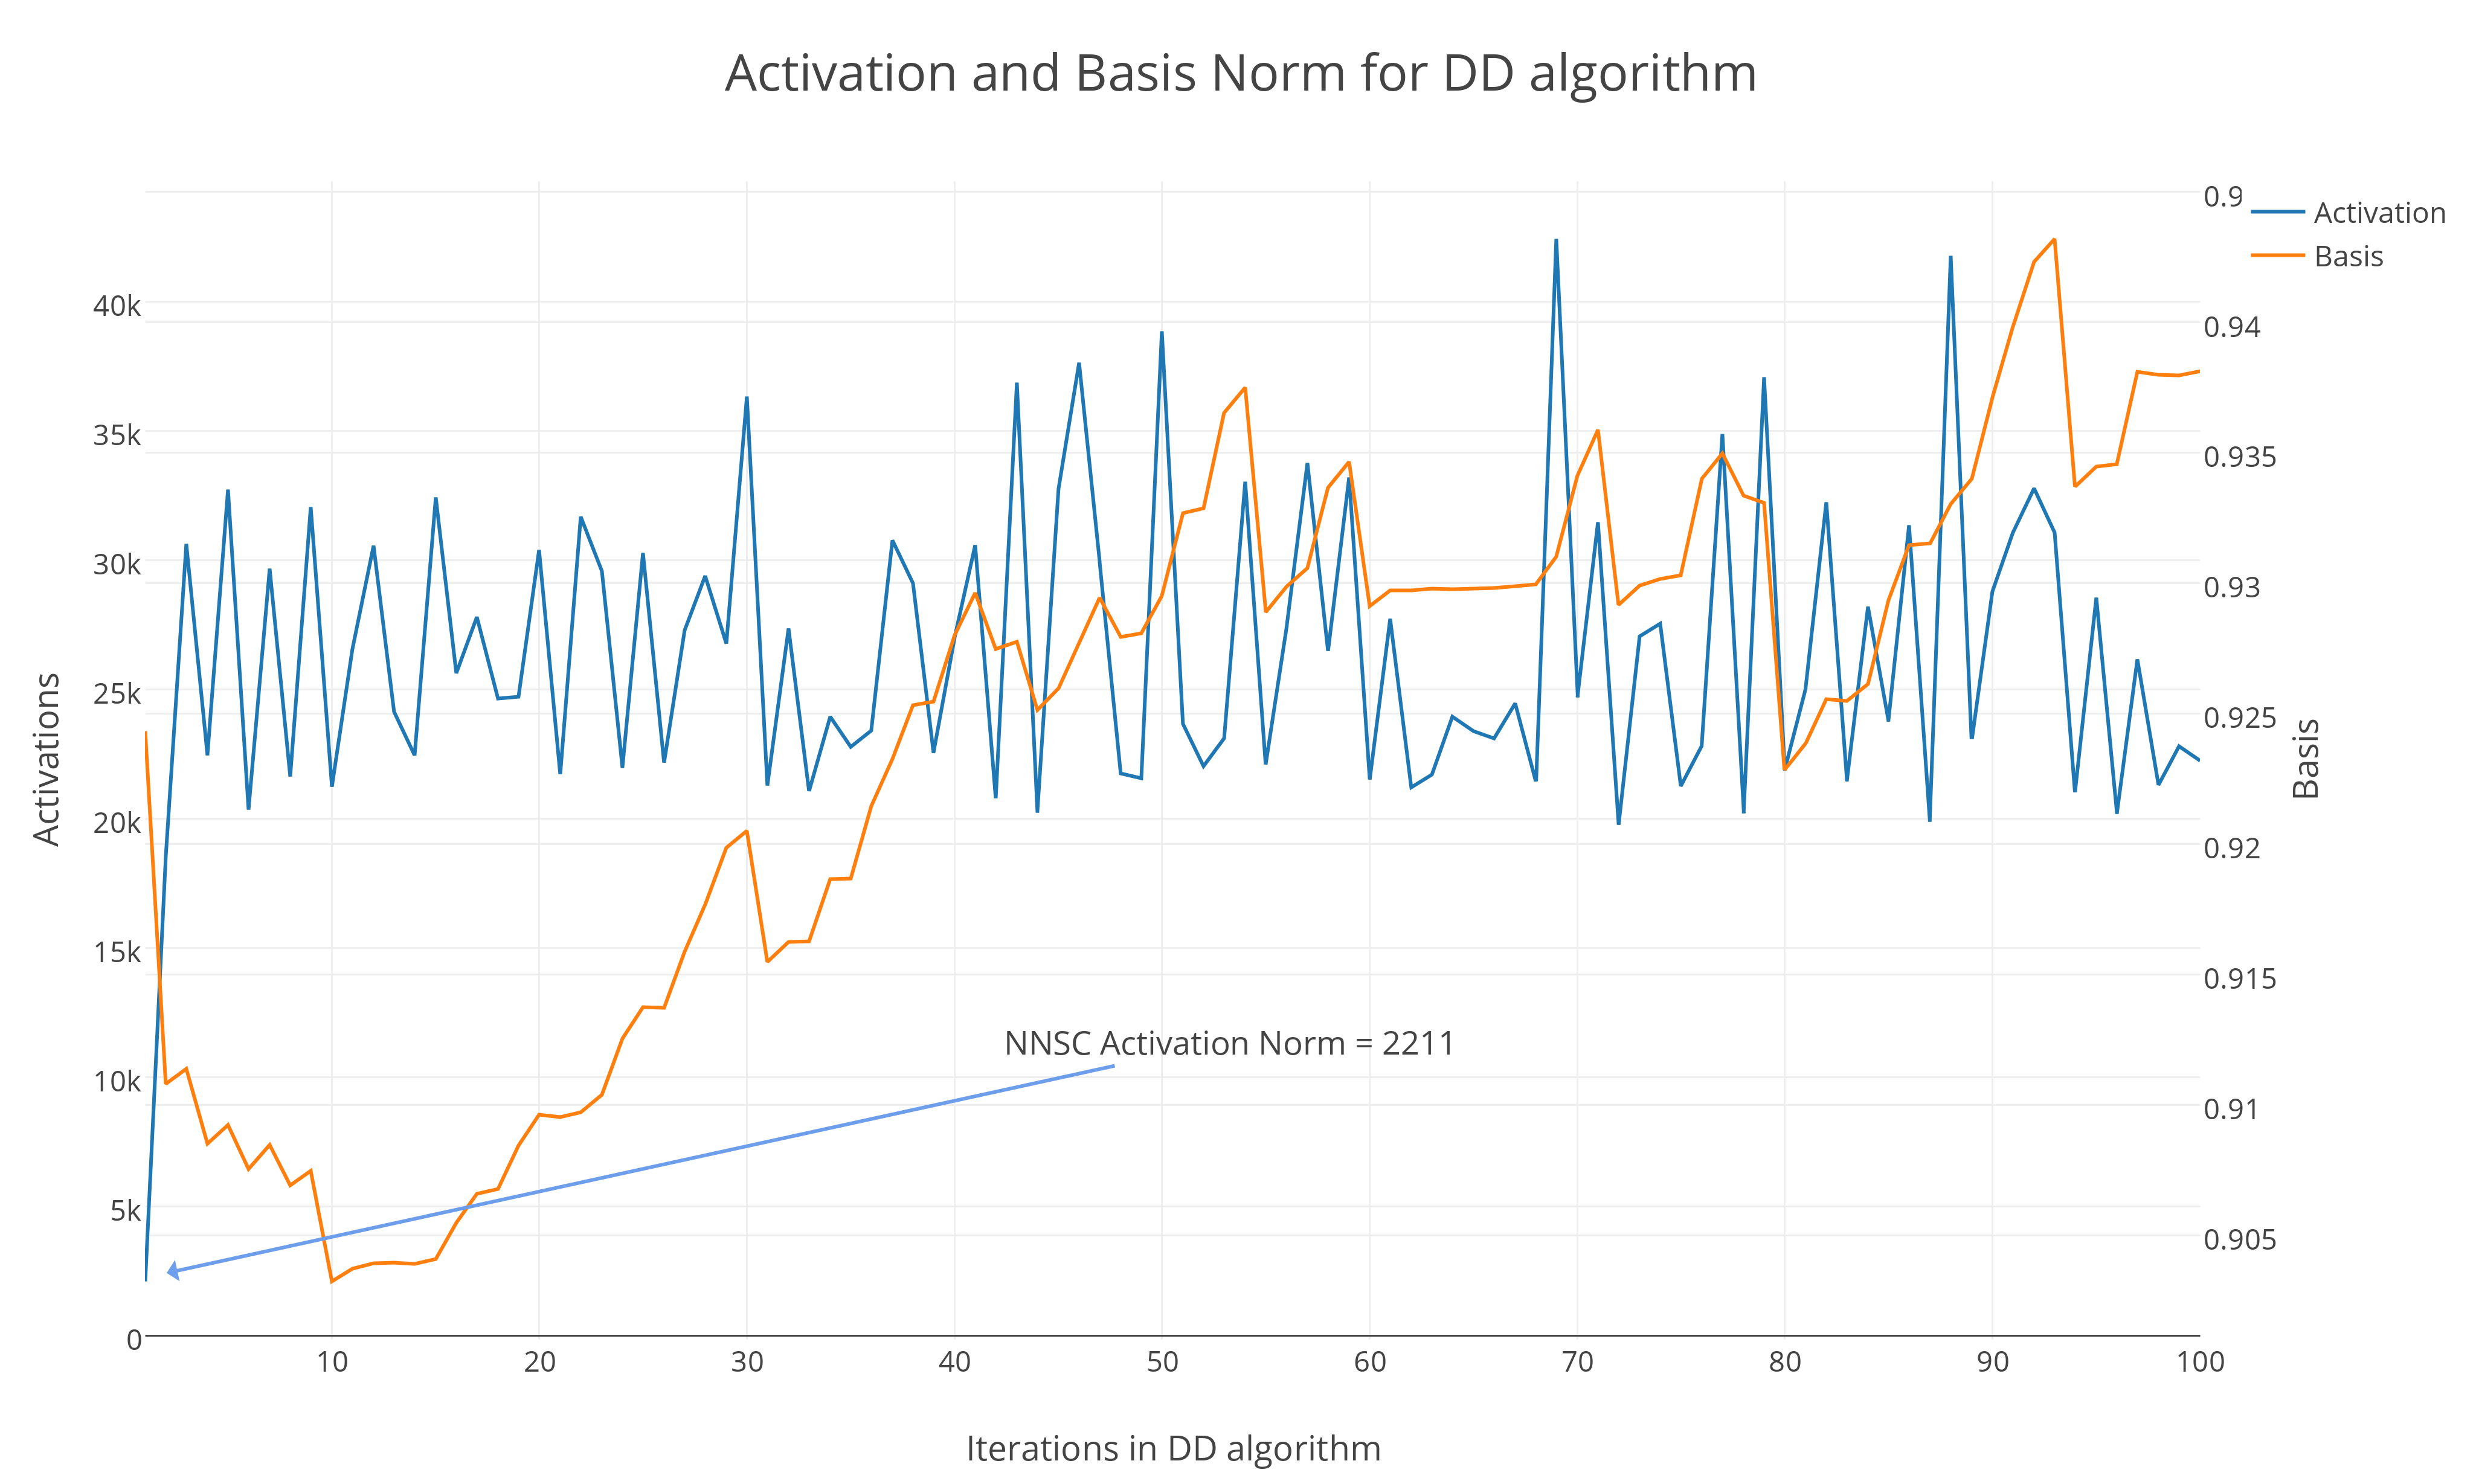
\includegraphics[scale=0.20]{./figures/a_b_norm.png}
	\note{
	The NNSC algorithm trains its activations separately for all of the appliances and yielded a norm of 2211 cumulatively for all of the appliances. We can see from the plot that when we start the DDSC algorithm the activation norms go from 2211 to around 25 000, which is probably due to the activations trying to adapt to the whole home energy consumption, which is vastly larger than each appliance. Interesting to note is that the basis norm slightly increases with each iteration, while the activations oscillate around 25 000. 
	The activations trained are not used for the predicting the values for a new dataset, from this iteration we only take out the basis matrix which seems to have adapted itself by changing from a norm of 0.925 to 0.94.
	}
\end{frame}
%%%%%%%%%%%%%%%%%%%%%%%%%%%%%%%%%%%%%%%%%%%%%
\begin{frame}
\frametitle{Accuracy and Error of the DDSC algorithm}
\framesubtitle{Result}
\begin{figure}
	\centering
	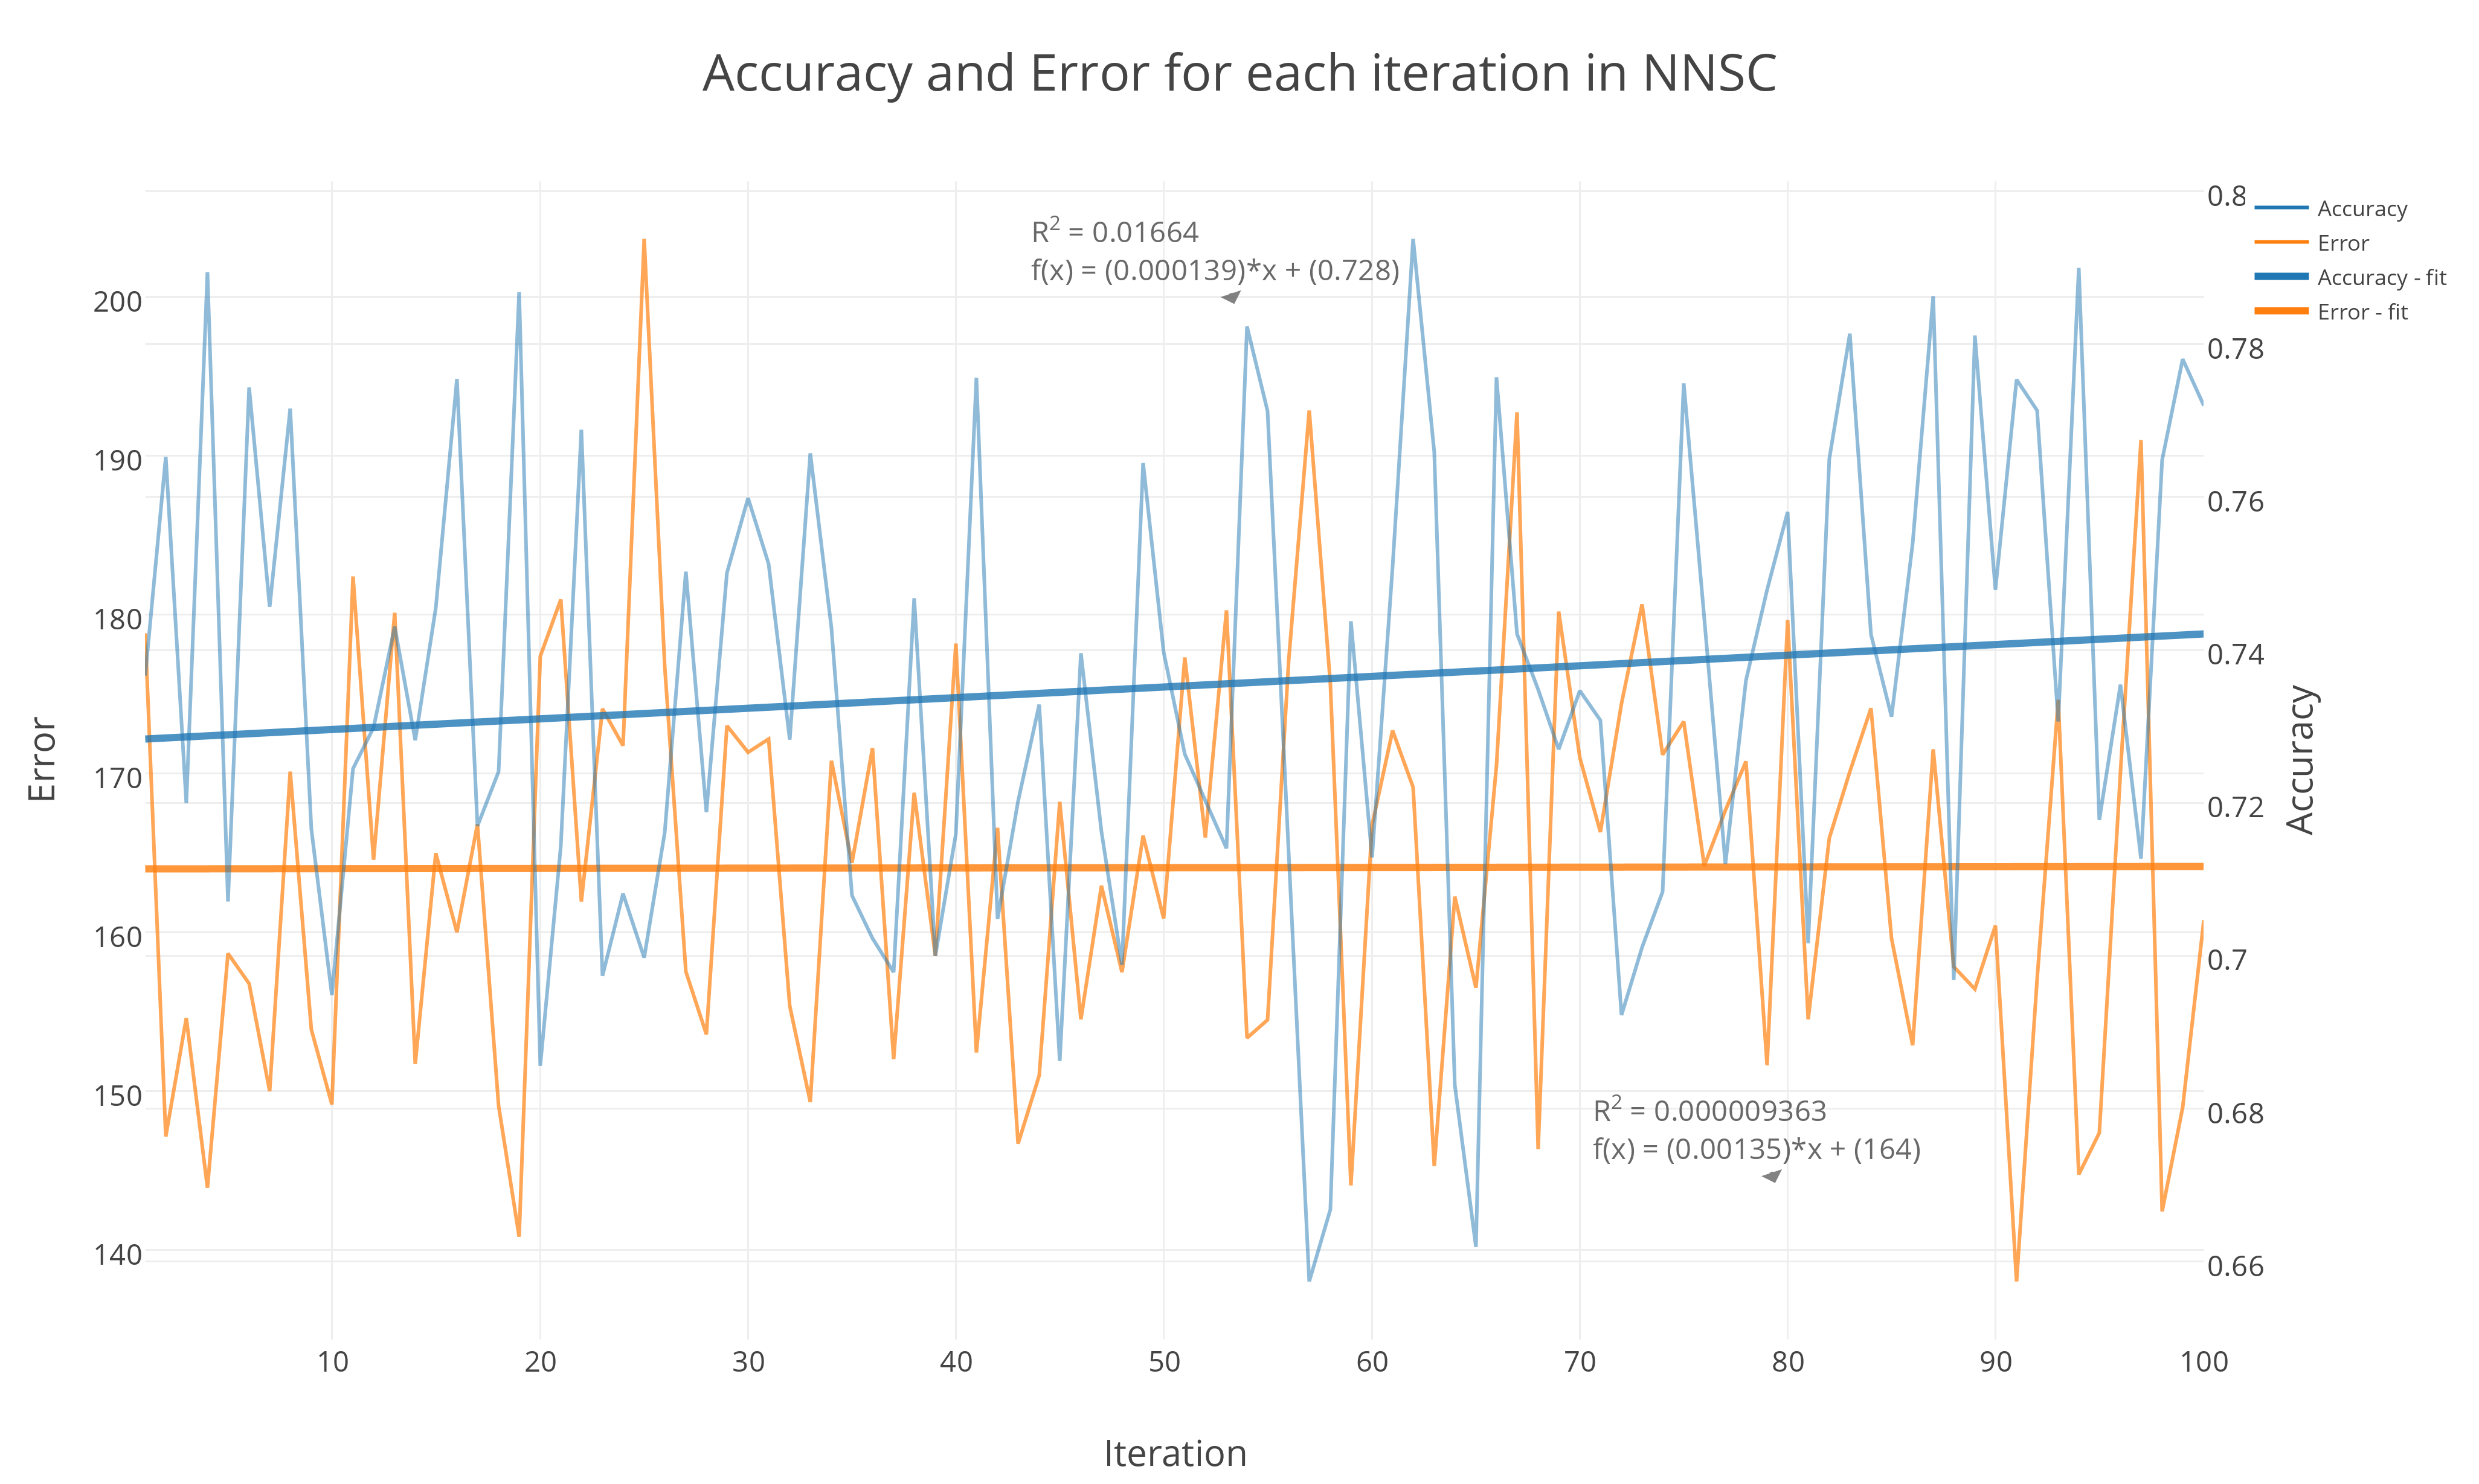
\includegraphics[scale=0.20]{./figures/acc_err_nnsc.png}
\end{figure}
\begin{equation*}
\text{Accuracy of Week} \equiv \frac{\sum_{i,q} \min \left\{ \sum_p ( \mathbf{X}_i)_{pq}, \sum_p ( \hat{\mathbf{B}}_i,\mathbf{A}_i)_{pq} \right\}}{\sum_{p,q} \bar{\mathbf{X}}_{p,q}}
\end{equation*}

\begin{equation*}
\text{Error } (\mathbf{X}_{1:k},\mathbf{B}_{1:k}) \vcentcolon= \sum_{i=1}^k \frac{1}{2} \norm{\mathbf{X}_i - \mathbf{B}_i \hat{\mathbf{A}}_i}_F^2,
\end{equation*}


\note{
	Figure 16 shows the disaggregation performance for the DDSC algorithm 4.5.2. It presents the disaggregation error from equation 27 on the left y-axis and the accuracy given in equation 32 on the right y-axis. Furthermore a linear regression has been done for both the error and accuracy. We note that the accuracy is around 35\% following the fitted line when the 100:th iteration has been done. From the figure we see that for each iteration, the algorithm has difficulty finding an optimal path towards a minimization as seen by the volatile behavior of both the error and accuracy. However, fitting a curve to the values, we see that the accuracy has a positive slope although with regards to a high variance for curve fitting, the plot shows that we cannot fully rely on the implementation due to its behavior. Investigating this further, we took a look at the activation and basis norms of the algorithm. This yielded the following figure.
	}
\end{frame}


%%%%%%%%%%%%%%%%%%%%%%%%%%%%%%%%%%%%%%%%%%%%%%%
\section{Future Work}
%%%%%%%%%%%%%%%%%%%%%%%%%%%%%%%%%%%%%%%%%%%%%%
\begin{frame}
	\frametitle{Extensions}
	\framesubtitle{DDSC}
	\begin{itemize}
		\item{Gridsearch across parameters; $\lambda,\alpha$}
		\item{Clustering - label data}
		\item{Adding extensions to the model, through Andrew}
	\end{itemize}
	Total energy priors: \\
	\vspace{0.1in}
	$F_{TEP}(\bar{\mathbf{X}},\mathbf{B}_{1:k},\mathbf{A}_{1:k}) = F(\bar{\mathbf{X}},\mathbf{B}_{1:k} \mathbf{A}_{1:k}) + \lambda_{TEP}\sum_{i=1}^k \norm{\mu_i\mathbf{1}^T-\mathbf{1}^T\mathbf{B}_i\mathbf{A}_i}^2_2$ \\
	\vspace{0.1in}
	Group Lasso: \\
	$F_{GL}(\bar{\mathbf{X}},\mathbf{B}_{1:k},\mathbf{A}_{1:k}) = F(\bar{\mathbf{X}},\mathbf{B}_{1:k} \mathbf{A}_{1:k}) + \lambda_{GL}\sum_{i=1}^k \sum_{j=1}^m \norm{\mathbf{a}_i^{(j)}}_2$ \\
\end{frame}
%%%%%%%%%%%%%%%%%%%%%%%%%%%%%%

\begin{frame}
	\frametitle{Recent work}
	\begin{itemize}
		\item{Dropouts, by Hinton et al. '14}% \cite{dropout}}
		\item{Hyperparameter Optimization}
		\item{Block Coordinate Update, '13}
		\item{Autoencoders, Google Cat '12, Deep Dream '14}% \cite{google}, Deep Dream}
		\item{Simple, Efficient, and Neural Algorithms for Sparse Coding '15}
		\item{Final word}
	\end{itemize}
		\note{
			Dropouts, where you randomly remove nodes; faster and more efficient. And adresses the problem of overfitting
			Hyperparameter optmization with baysian
			The problem is nonconvex but is convex is each block
			Autoencoders by Google
			
			would people want to leave their energy consumption in public?
			cause it will.}
\end{frame}
%%%%%%%%%%%%%%%%%%%%%%%%%%%

\begin{frame}
\begin{center}
\huge
Thank you!
\normalsize \\
\vspace{0.3in}
Questions?
\end{center}
\end{frame}
%
%\begin{frame}
%	\frametitle{Citations}
%	\begin{thebibliography}
%		
%		\bibitem{dropout}
%		Nitish Srivastava, Geoffrey Hinton, Alex Krizhevsky, Ilya Sutskever, and Ruslan Salakhutdinov.
%		\emph{Dropout: A simple way to prevent neural networks from overfitting}. JMLR, 2014.
%		
%		\bibitem{google}
%		Le, Q., Ranzato, M., Monga, R., Devin, M., Chen, K., Corrado, G., et al. \emph{Building high-level features using large scale unsupervised learning}. In ICML, 2012.
%		
%		
%	\end{thebibliography}
%\end{frame}

\egroup
\end{document}
